\documentclass[addpoints,12pt]{exam} %answers 
\usepackage[paper=a4paper,left=15mm,right=15mm,top=25mm,bottom=25mm]{geometry}
\usepackage{graphicx}
%\usepackage[dvips]{graphicx}
\usepackage{floatflt,epsfig} 
\usepackage{ngerman}
\usepackage{german}
\usepackage[utf8]{inputenc}
\usepackage{amssymb, amsmath}
\usepackage[gate,ic,optics]{circ}
\usepackage{hyperref}

\usepackage{tikz,pgfplots}

\usepackage{graphicx}
%\usepackage{geometry}
\usepackage{calc}


\usepackage{qrcode} 
\usepackage{wrapfig}
\usepackage{gensymb}
\usepackage{siunitx}

\usepackage{color}
\definecolor{GridColor}{gray}{0.8}
\definecolor{SolutionBoxColor}{gray}{0.8}
\definecolor{SolutionColor}{rgb}{0.8,0.9,1}

\colorgrids
\colorsolutionboxes

%%MACROS 
\newcommand{\tdate}{12. November 2021}
\newcommand{\myqr}{\qrcode[hyperlink, height = 1cm]{https://upload.wikimedia.org/wikipedia/commons/d/d8/Entscheidungsbaum_zur_Konvergenz_und_Divergenz_von_Reihen.svg}}
\newcommand\gauss[2]{1/(#2*sqrt(2*pi))*exp(-((x-#1)^2)/(2*#2^2))} % Gauss function, parameters mu and sigma
%%
\newcommand{\gr}{ETIT-1}

\sisetup{
locale = DE ,
per-mode = symbol
}

\pagestyle{headandfoot}

\headrule
\footrule
\firstpageheader{\gr}{\bfseries\Large {Übungsblatt 4}}{\tdate}
\runningheader{\gr}
{Übungsblatt - 4}
{\tdate}
\firstpagefooter{\gr}{Seite \thepage\ von \numpages}{\myqr}
\runningfooter{\gr}{Seite \thepage\ von \numpages}{\myqr}

\boxedpoints
%\pointpoints{Punkt}{Punkte}
\pointsinmargin
\marginpointname{\%}

\begin{document}
%\setcounter{section}{1} %current page -1
\author{Shah Rrks}
\section*{Mathe}
\section*{Konvergenz und Divergenz von Reihen}
\begin{questions}
\question Untersuchen Sie die folgenden Reihen auf Konvergenz bzw. Divergenz, bestimmen
Sie falls möglich den Wert der Reihe. (Quelle: Höhere Mathematik in Rezepten)

\begin{figure}[h]
    \centering
    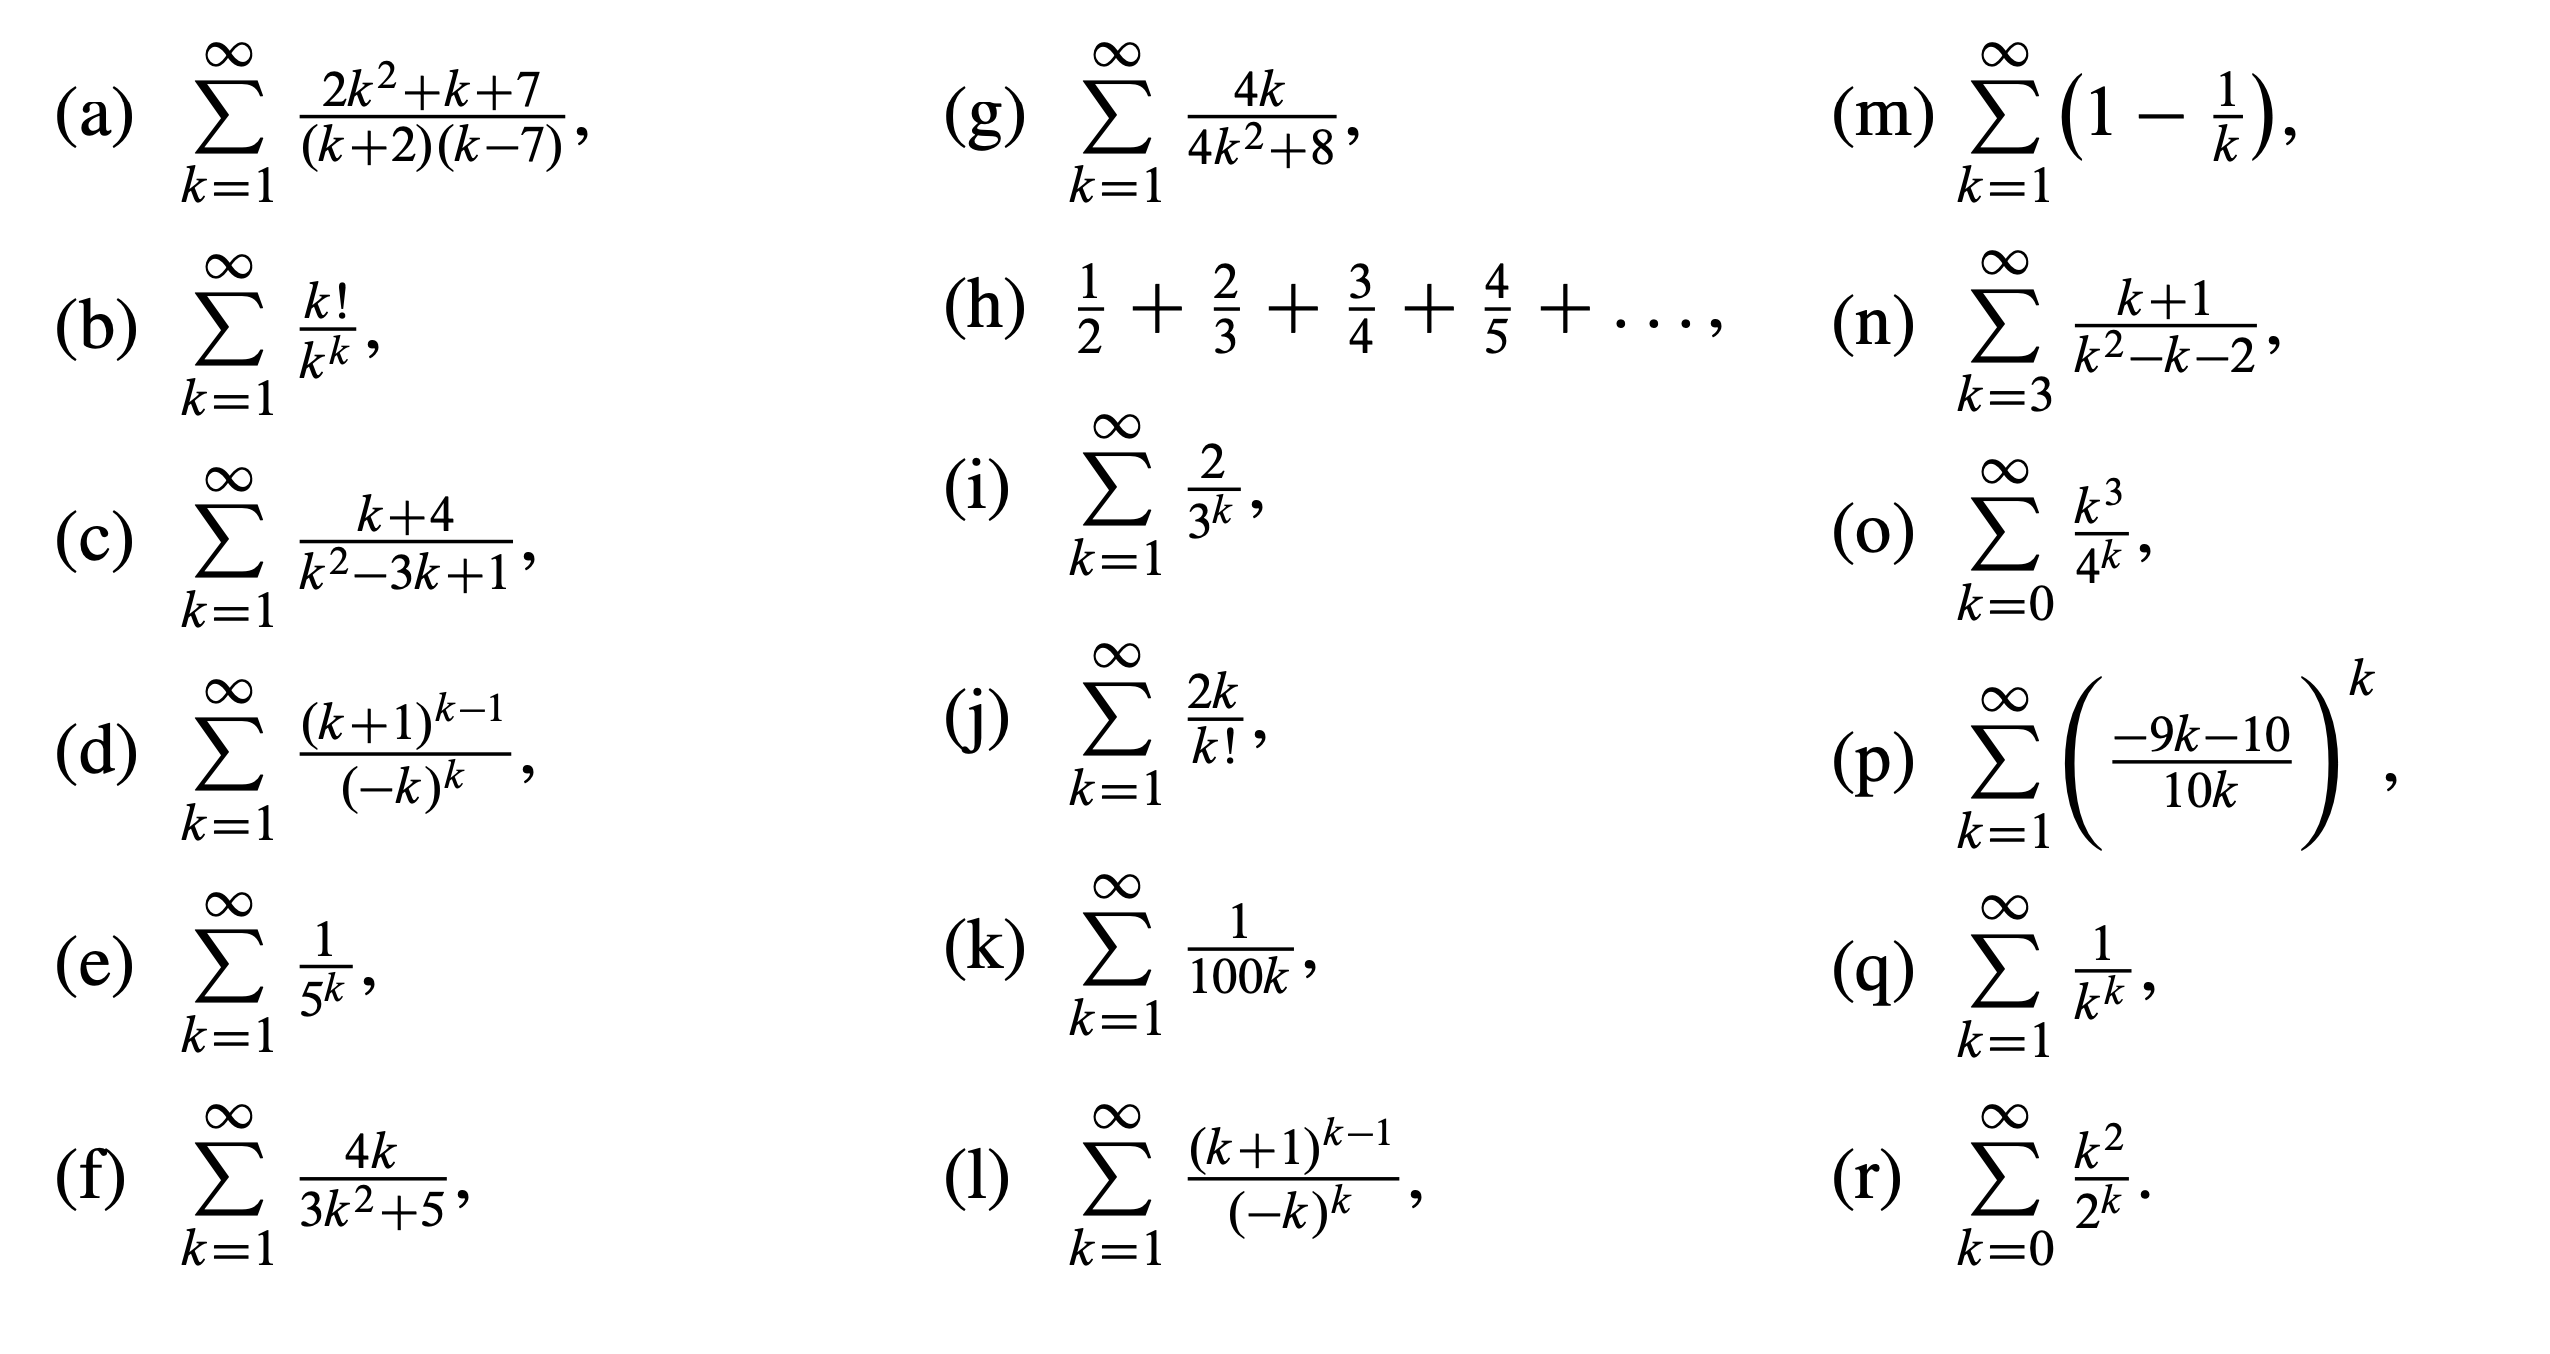
\includegraphics[width=0.8\textwidth]{auf1.png}
\end{figure}

\end{questions}



\begin{figure}[h]
\centering
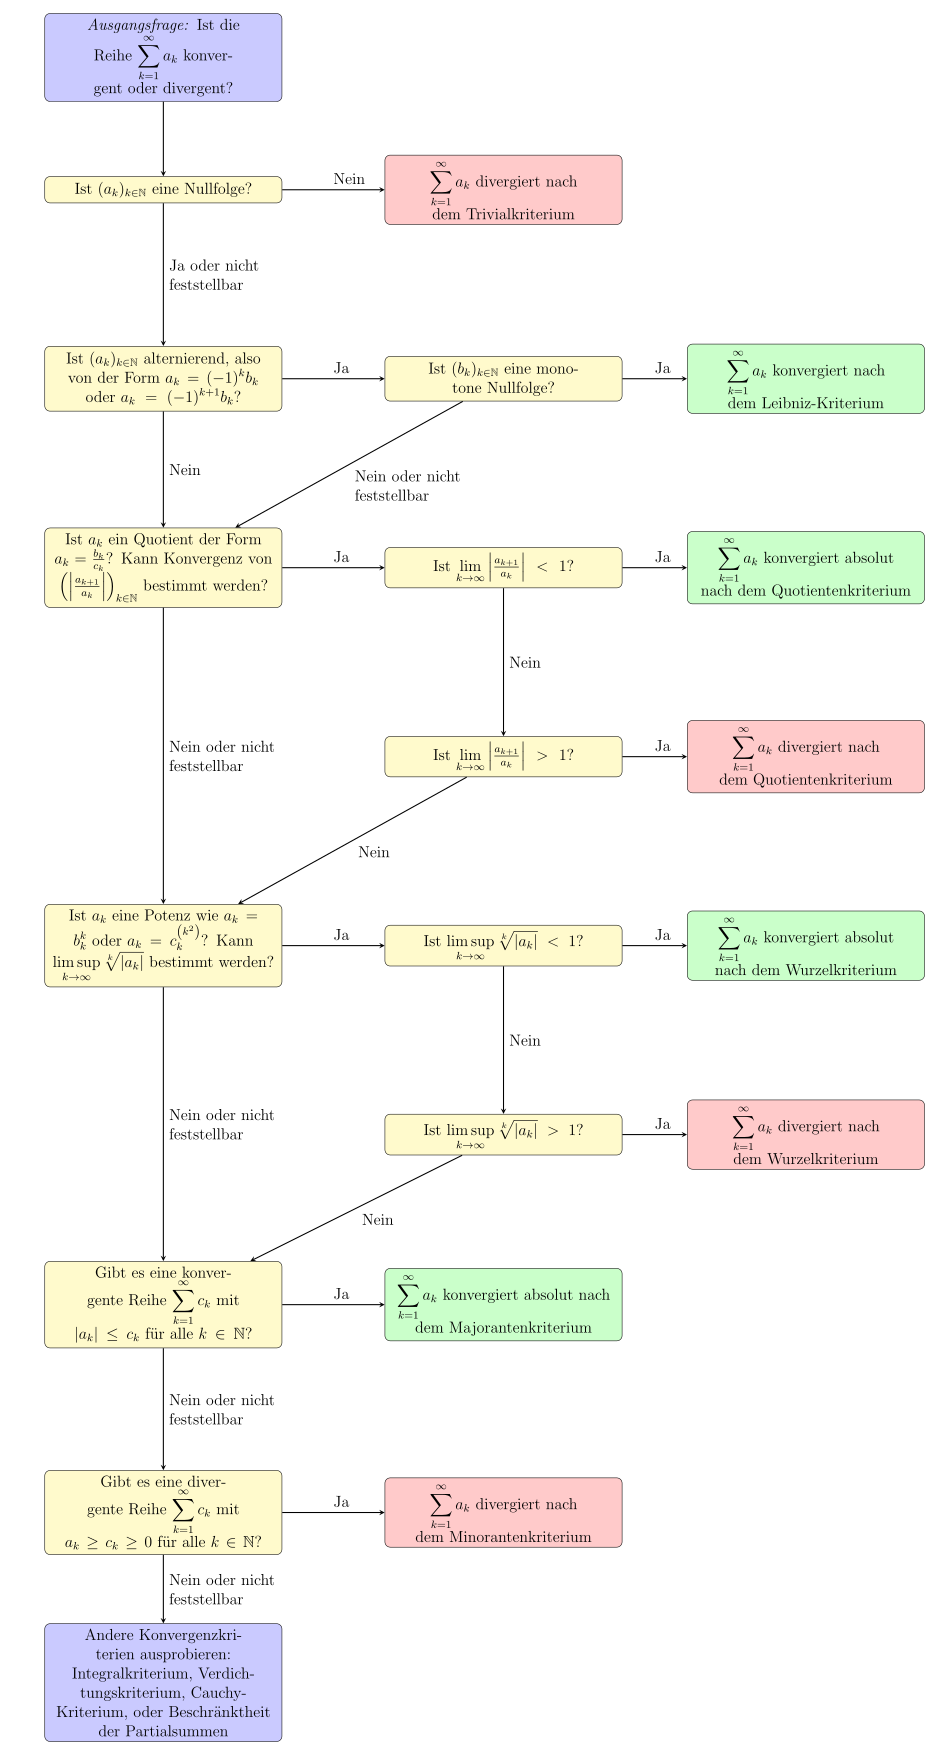
\includegraphics[width=0.7\textwidth]{algorithm.png}
\caption{Konvergez und Divergenz von Reihen}
\label{fig:Konvergez und Divergenz von Reihen}
Quelle : Mathe für nicht freaks 

\end{figure}


\end{document}